\documentclass[newpage,hints,handout]{ximera}

\usepackage{microtype}
\usepackage{tikz}
\usepackage{tkz-euclide}
\usetkzobj{all}
\tikzstyle geometryDiagrams=[ultra thick,color=blue!50!black]

\renewcommand{\epsilon}{\varepsilon}



\title{Hyperbolic lunes and triangles}

\begin{document}
\begin{abstract}
In this activity, we explore the areas of lunes and triangles in
hyperbolic geometry.
\end{abstract}
\maketitle

We know that the area of a triangle on the $R$-sphere with angles
$\alpha$, $\beta$, and $\gamma$ is given by
\[
R^2(\alpha+\beta+\gamma - \pi).
\]
\begin{problem}
  Briefly sketch the line of reasoning used to deduce the formula for
  the area of a triangle on the $R$-sphere.
\end{problem}

We will use similar reasoning to deduce the formula for the area of a triangle
with angles $\alpha$, $\beta$, and $\gamma$ in hyperbolic geometry.

\section{Hyperbolic lunes}

Consider the following diagram on the Klein disk, that is the central projection
of hyperbolic geometry:
\begin{image}
  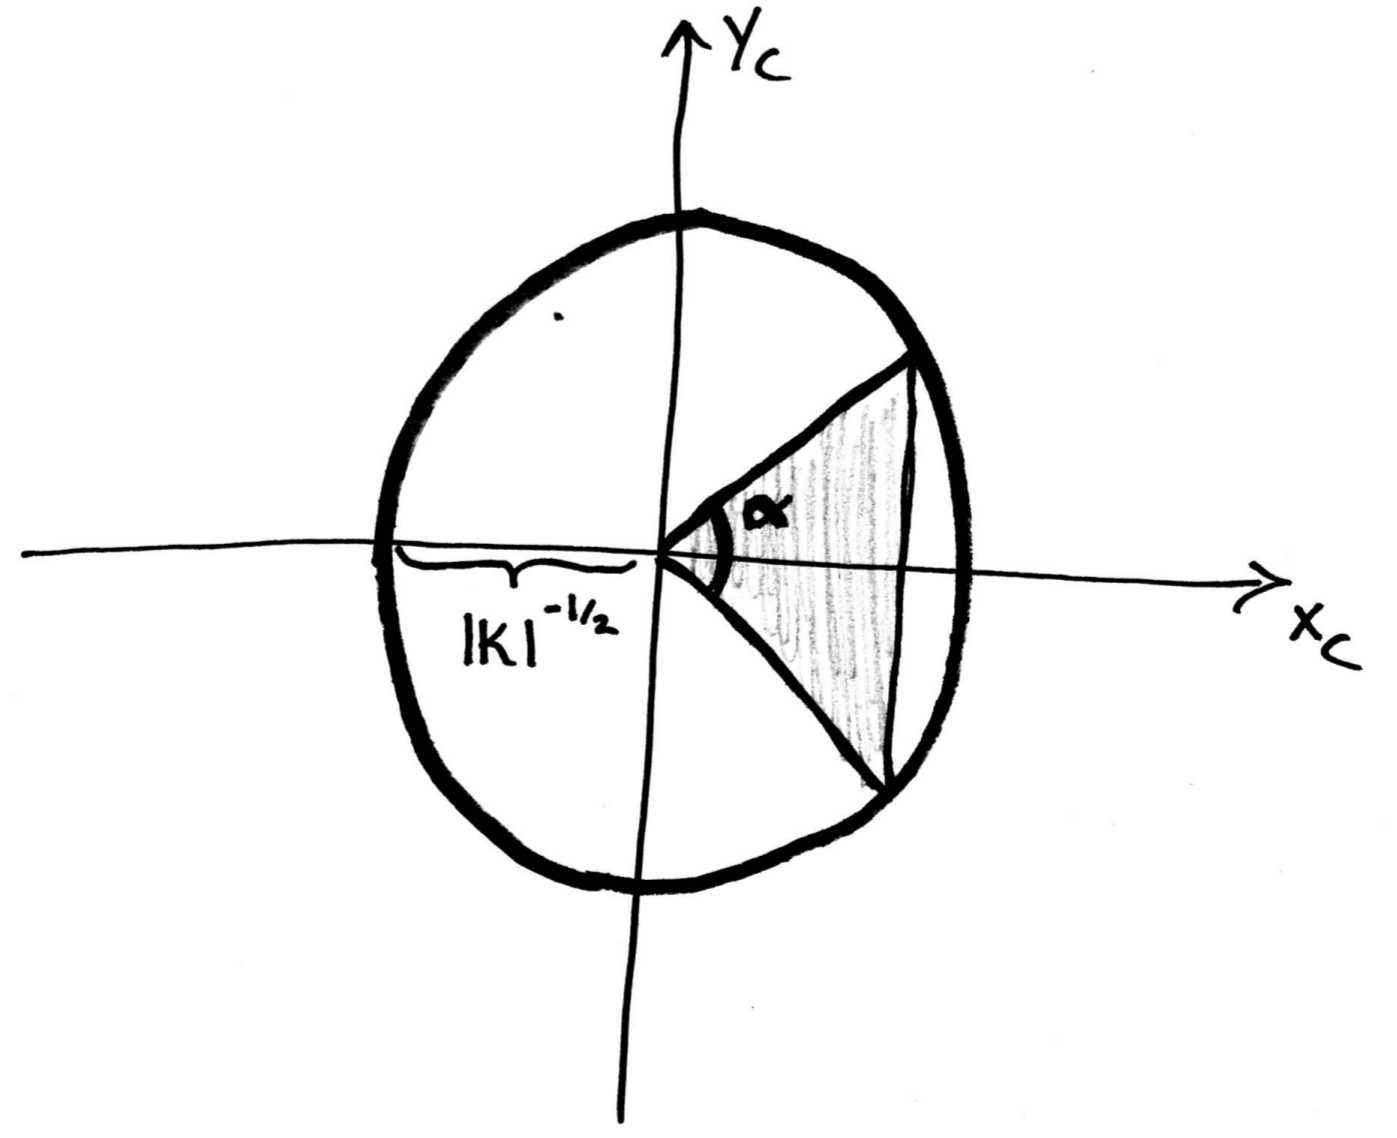
\includegraphics[width=3in]{diagramOfHyperbolicLune.png}
\end{image}

Notice that in both the Klein model and the Poincar\'e model, every line hits
``the circle at infinity'' at two specific points.  This means we can talk about
shapes with ``vertices at infinity''.

\begin{definition}
  We define an \dfn{$\boldsymbol\alpha$-lune} in hyperbolic geometry to be a
  triangle with an angle of measure $\alpha$ where vertices opposite of $\alpha$
  are at infinity.
\end{definition}

We have seen that
\begin{align*}
  \iint_{L_c} \sqrt{
  \det
  \begin{bmatrix}
    \pp[X]{x_c}\bullet_K \pp[X]{x_c} & \pp[X]{y_c}\bullet_K \pp[X]{x_c} \\
    \pp[X]{x_c}\bullet_K \pp[X]{y_c} & \pp[X]{y_c}\bullet_K \pp[X]{y_c}
  \end{bmatrix}
  }\d x_c\d y_c &=
  \iint_{L_c} \sqrt{\det P_c}\d x_c\d y_c\\
  &=\iint_{L_c} \left(K\left(x_c^2+y_c^2\right)+1\right)^{-3/2} \d x_c\d y_c.
\end{align*}


In what follows, we will assume that $K=-1$. This will simplify the
computations somewhat. Once the mathematician is familiar with this
case, the general case when $K<0$ will fall easily.


\begin{problem}
  Convert
  \[
  \iint_{L_c} \left(-\left(x_c^2+y_c^2\right)+1\right)^{-3/2} \d x_c\d y_c
  \]
  to polar coordinates and compute the integral.
  \begin{hint}
    Redraw the picture above with $\alpha = 2\beta$ and $K=-1$.
  \end{hint}
  \begin{hint}
    Recall that to convert to polar coordinates, set
    \begin{align*}
      r &= \sqrt{x_c^2+y_c^2},\\
      \theta &= \arctan(y_c/x_c),
    \end{align*}
    and replace $\d x_c\d y_c$ with $r\d r\d \theta$.
  \end{hint}
  \begin{hint}
    At some point you may wish to use the following identities:
    \[
    \begin{split}
      \cos^2\theta + \sin^2\theta &=1\\
      \cos^2\theta &= 1-\sin^2\theta
    \end{split}
    \qquad
    \begin{split}
      \cos^2\beta + \sin^2\beta &=1\\
      \cos^2\beta &= 1-\sin^2\beta
    \end{split}
    \]
    So
    \begin{align*}
      \cos^2\theta - \cos^2\beta &= 1 - \sin^2\theta - \left(1-\sin^2\beta\right)\\
      &= \sin^2\beta - \sin^2\theta.       
    \end{align*}
  \end{hint}
  \begin{hint}
    It may also be helpful to recall that when $a>0$,
    \[
    \int \frac{1}{\sqrt{a - u^2}} \d u = \arcsin\left(\frac{u}{\sqrt{a}}\right) + C.
    \]
  \end{hint}
  \begin{hint}
    Finally, as a gesture of friendship, I will tell you that you will
    (hopefully!) deduce that this integral equals $\pi-\alpha$.
  \end{hint}
  \begin{freeResponse}
    Write
    \[
    \int_{L_c} \left(-\left(x_c^2+y_c^2\right)+1\right)^{-3/2} \d x_c\d y_c
    = \int_{-\beta}^\beta \int_0^{\frac{\cos \beta}{\cos\theta}}\left(-r^2+1\right)^{-3/2} r\d r\d \theta.
    \]
    Integrating this from the inside-out we find
    \begin{align*}
      &= \int_{-\beta}^\beta \eval{\left(-r^2+1\right)^{-1/2}}_0^{\frac{\cos \beta}{\cos\theta}}\d \theta\\
      &= \int_{-\beta}^\beta \left(-\left(\frac{\cos \beta}{\cos\theta}\right)^2+1\right)^{-1/2}\d\theta - \eval{\theta}_{-\beta}^\beta\\
      &= \int_{-\beta}^\beta \left(1-\frac{\cos^2 \beta}{\cos^2\theta}\right)^{-1/2}\d \theta -2\beta\\
      &= \int_{-\beta}^\beta \left(\frac{\cos^2\theta - \cos^2 \beta}{\cos^2\theta}\right)^{-1/2} \d \theta-\alpha\\
      &= \int_{-\beta}^\beta \frac{\cos\theta}{\sqrt{\cos^2\theta - \cos^2 \beta}}\d \theta - \alpha.
    \end{align*}
    Now apply a trigonometric substitution,
    \[
    = \int_{-\beta}^\beta \frac{\cos\theta}{\sqrt{\sin^2\beta - \sin^2 \theta}}\d \theta- \alpha,
    \]
    Using the hint above we see
    \begin{align*}
      &= \eval{\arcsin\left(\frac{\sin\theta}{\sin\beta}\right)}_{-\beta}^\beta - \alpha\\
      &= \arcsin\left(\frac{\sin\beta}{\sin\beta}\right)- \arcsin\left(\frac{\sin(-\beta)}{\sin\beta}\right)- \alpha\\
      &= \arcsin(1)-\arcsin(-1)-\alpha\\
      &= \frac{\pi}{2}-\frac{-\pi}{2}-\alpha\\
      &= \pi-\alpha.
    \end{align*}
  \end{freeResponse}
\end{problem}


\section{Hyperbolic triangles}

Again assuming $K=-1$, we will use our knowledge that the hyperbolic
$\alpha$-lune has area $\pi-\alpha$ to compute the area of an
\textit{ideal triangle} in hyperbolic geometry. Note, now we are working under
stereographic projection in the Poincar\'e disk (because it's more fun to draw.)

\begin{definition}
  An \dfn{ideal triangle} is a triangle in hyperbolic geometry with all of
  its vertices at infinity.
\end{definition}

\begin{problem}
  Use the diagrams below
  \begin{image}
  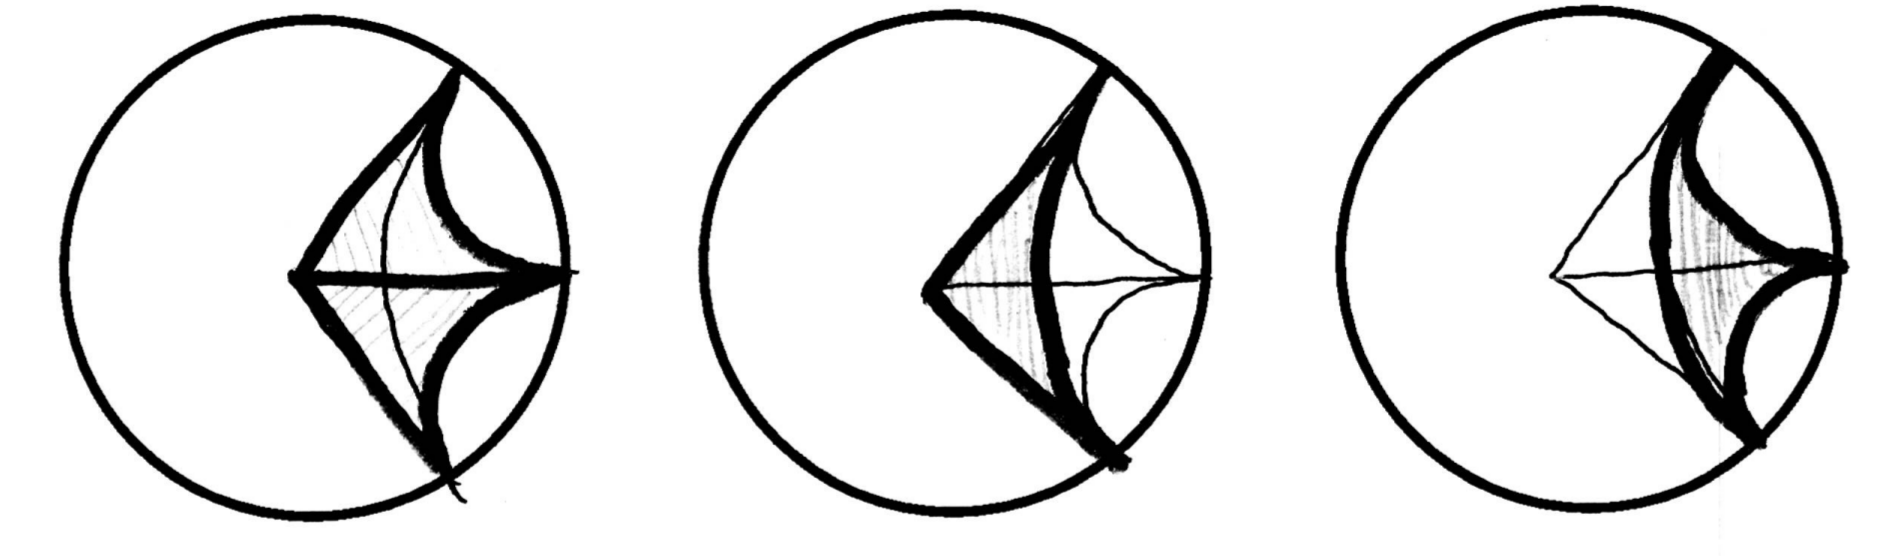
\includegraphics[width=4in]{diagramOfIdealTri.png}
  \end{image}
  to help compute the area of an ideal triangle in hyperbolic geometry.
  \begin{hint}
    Above we see a comic-strip of Poincar\'e disks.
  \end{hint}
  \begin{hint}
    Make sure your computation is general.  That is, start with an arbitrary
    ideal triangle and then fill in the rest of the diagram.
  \end{hint}
\end{problem}


\begin{definition}
  An \dfn{ideal $\boldsymbol{n}$-gon} is an $n$-gon in hyperbolic
  geometry with its vertices at infinity.
\end{definition}

\begin{problem}
Use induction to derive a formula for the area of any ideal $n$-gon in
hyperbolic geometry.
\end{problem}

\begin{problem}
  Use the diagrams below
  \begin{image}
  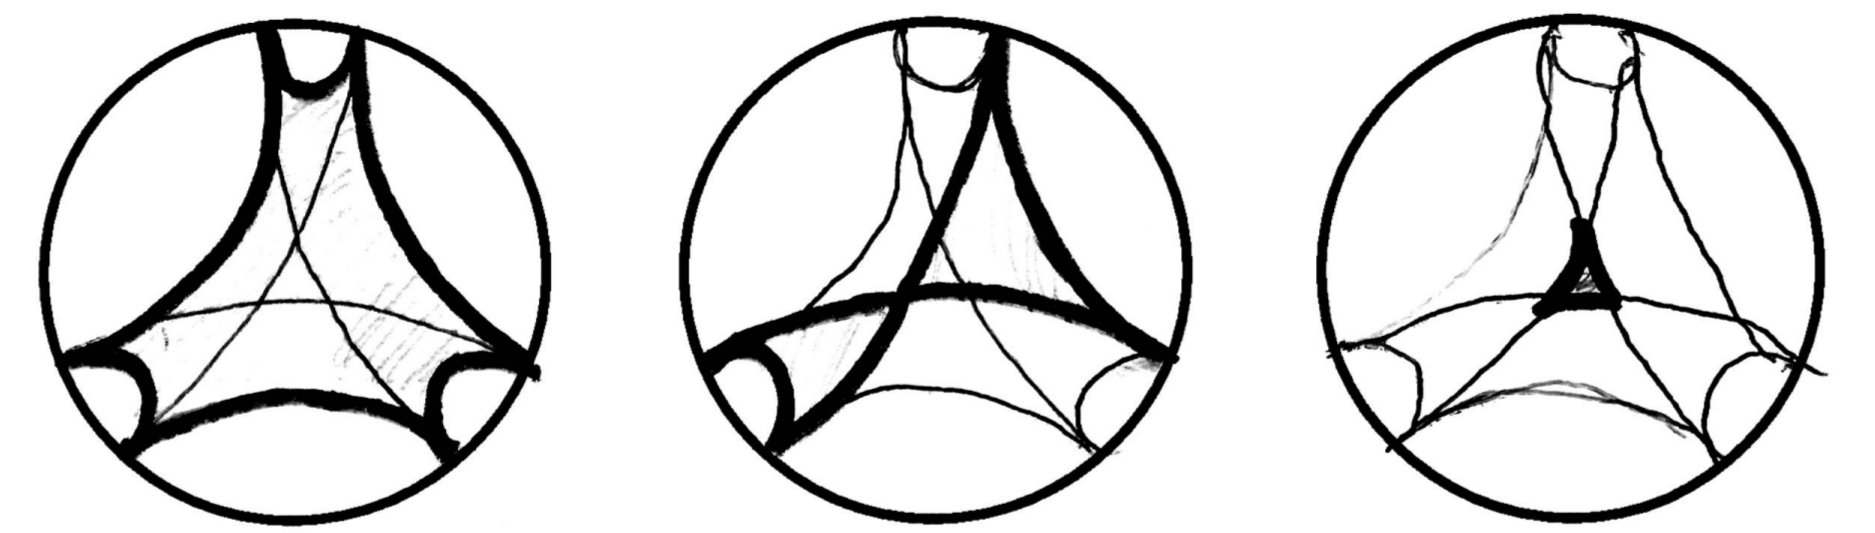
\includegraphics[width=4in]{diagramHex.png}
  \end{image}
  to help compute the area of a triangle in hyperbolic geometry.
  \begin{hint}
    Make your own drawings inspired by those above.
  \end{hint}
  \begin{hint}
    Make sure your computation is general: start with an arbitrary triangle and
    explain how you can fill in the rest of the diagram.
  \end{hint}
\end{problem}


\begin{problem}
Summarize the results from this section. In particular, indicate which
results follow from the others.
\begin{freeResponse}
\end{freeResponse}
\end{problem}




\end{document}
